\subsubsection*{Comprendere i dati: il ruolo della gravità e dell'attrito}

La produzione e l'analisi dei filmati offre permette di allargare molto l'osservazione,  controllando numericamente molti particolari, tuttavia una comprensione approfondita di una fenomenologia richiede una attività di sintesi che, fino a questo monento non è ancora compiuta.\newline

Riprendendo lo schema a tre colonne: "Cosa faccio", "Cosa osservo", "Come spiego", si può riconoscere facilemente che l'ultima delle tre colonne, fino ad ora, non è stata sviluppata in modo esaustivo.\newline
Probabilmente, l'unica con conclusione che, al momento, viene spontaneo acquisire è che il piano del banco non è perfettamente orrizzontale, a causa delle differenze osservate nel moto di discesa e quello di salita.\newline

Tuttavia, i grafici possono dire qualcosa in più. Perché il moto in salita è un moto accelerato, mentre quello in discesa è quasi perfettamente costante. Quali sono le {\bf cause} che determinano l'accelarazione o il moto uniforme?\newline

L'inclinazione del piano, ad esempio, non è sufficiente. Possiamo accettare che la pila sia frenata per gravità in salita, ma dovremmo aspettarci, durante la discesa, una accelerazione uguale e contraria. Se invece il moto è uniforme, significa che il sistema è affetto da qualche causa di accelerazione differente. In effetti, sebbene la pila sia un oggetto cilindrico, è frenata da qualche forma di attrito. Anzi, a pensarci bene, se non ci fosse un attrito non potrebbe neppure rotolare, ma traslerebbe rigidamente come un oggetto in volo libero sopra il tavolo. La rotazione, di conseguenza, è possibile solo se il piano funge da punto di appoggio per il cilindro.\newline

Possiamo affermare, dunque, che gli elementi necessari per descrivere le cause del moto della pila sono:\newline
\begin{itemize}
\item {la velocità;}
\item {la accelerazione verso il basso, associata alla gravità;}
\item {la decelerazione di attito, opposta alla velocità;}
\end{itemize}

Trattandosi di grandezze vettoriali possono essere rappresentate graficamente in questo modo:

\begin{figure}[H]
 \centering
 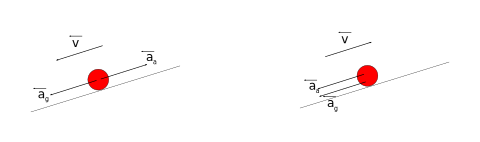
\includegraphics[width=.7\textwidth]{../immagini/leCauseDelMotoDellaPila.png}
 \label{fig:causeDelMotoDellaPila}
\end{figure}

Dalla figura, possiamo osservare che i fattori che determinano il comportamento della pila, cioè la gravità e l'attrito, si sovrappongono in modo differente durante la salita e durante la discesa, e questo può spiegare perché uno dei moti è accelerato mentre l'altro no. Adesso siamo in grado di riscrivere il nostro schema a tre colonne in un modo migliore che in precedenza:

\begin{center}
\begin{tabular}{||*{3}{p{5cm}|}|}
\hline
Cosa faccio & Cosa osservo & Come spiego \\
\hline

Una pila viene lanciata lungo un piano inclinato con una velocità iniziale modesta, prima in una direzione e poi nell'altra. &
Nella prima direzione si osserva un moto che si mantiene rettilineo uniforme per un lungo tratto.\newline
Nella seconda direzione, invece, il moto è soggetto a una visibile accelerazione negativa. &
Le due osservazioni fanno pensare che il rotolamento dipende da due cause diverse. La prima è la forza di gravità, che determina un'accelerazione verso il basso, la seconda è l'attrito tra la pila e il piano. Le due forze si sovrappongono in modo {\slshape \bf costruttivo} durante la salita e {\slshape \bf distruttivo} durante la discesa. Il fatto che il moto di discesa sia pressoché uniforme fa pensare che queste due forze debbano avere la stessa intensità. \\
\hline
\end{tabular}
\end{center}

Se chiamiamo $a_s$ l'accelerazione misurata in salita, e se poniamo uguale a zero l'accelerazione osservata in discesa, $a_g$ l'accelerazione associata alla gravità ed $a_a$ l'accelerazione dovuta all'attrito, possiamo stabilire la seguente relazione:

\begin{center}
\begin{math}
\left\{
\begin{array}{r}
a_m = a_g + a_a \\
0 = a_g - a_a
\end{array}
\right.
\end{math}
\end{center}

